% adding the line below for Multifile document support with LatexTools Sublime package 
%!TEX root = manuscript.tex


% Results

\section{Results}

\subsection{Systematic review}

Search terms entered in Pubmed returned 152 results during the last check on December 14, 2017 and 28 articles included in previous
 meta-analysis on \gls{nfb} were identified. After the selection process illustrated in \cref{Figure:systematic_review_workflow}, 
31 studies were included in the factors analysis and 15 in the update of \citet{Cortese2016}. 

\begin{figure}[h!]
  \centering
  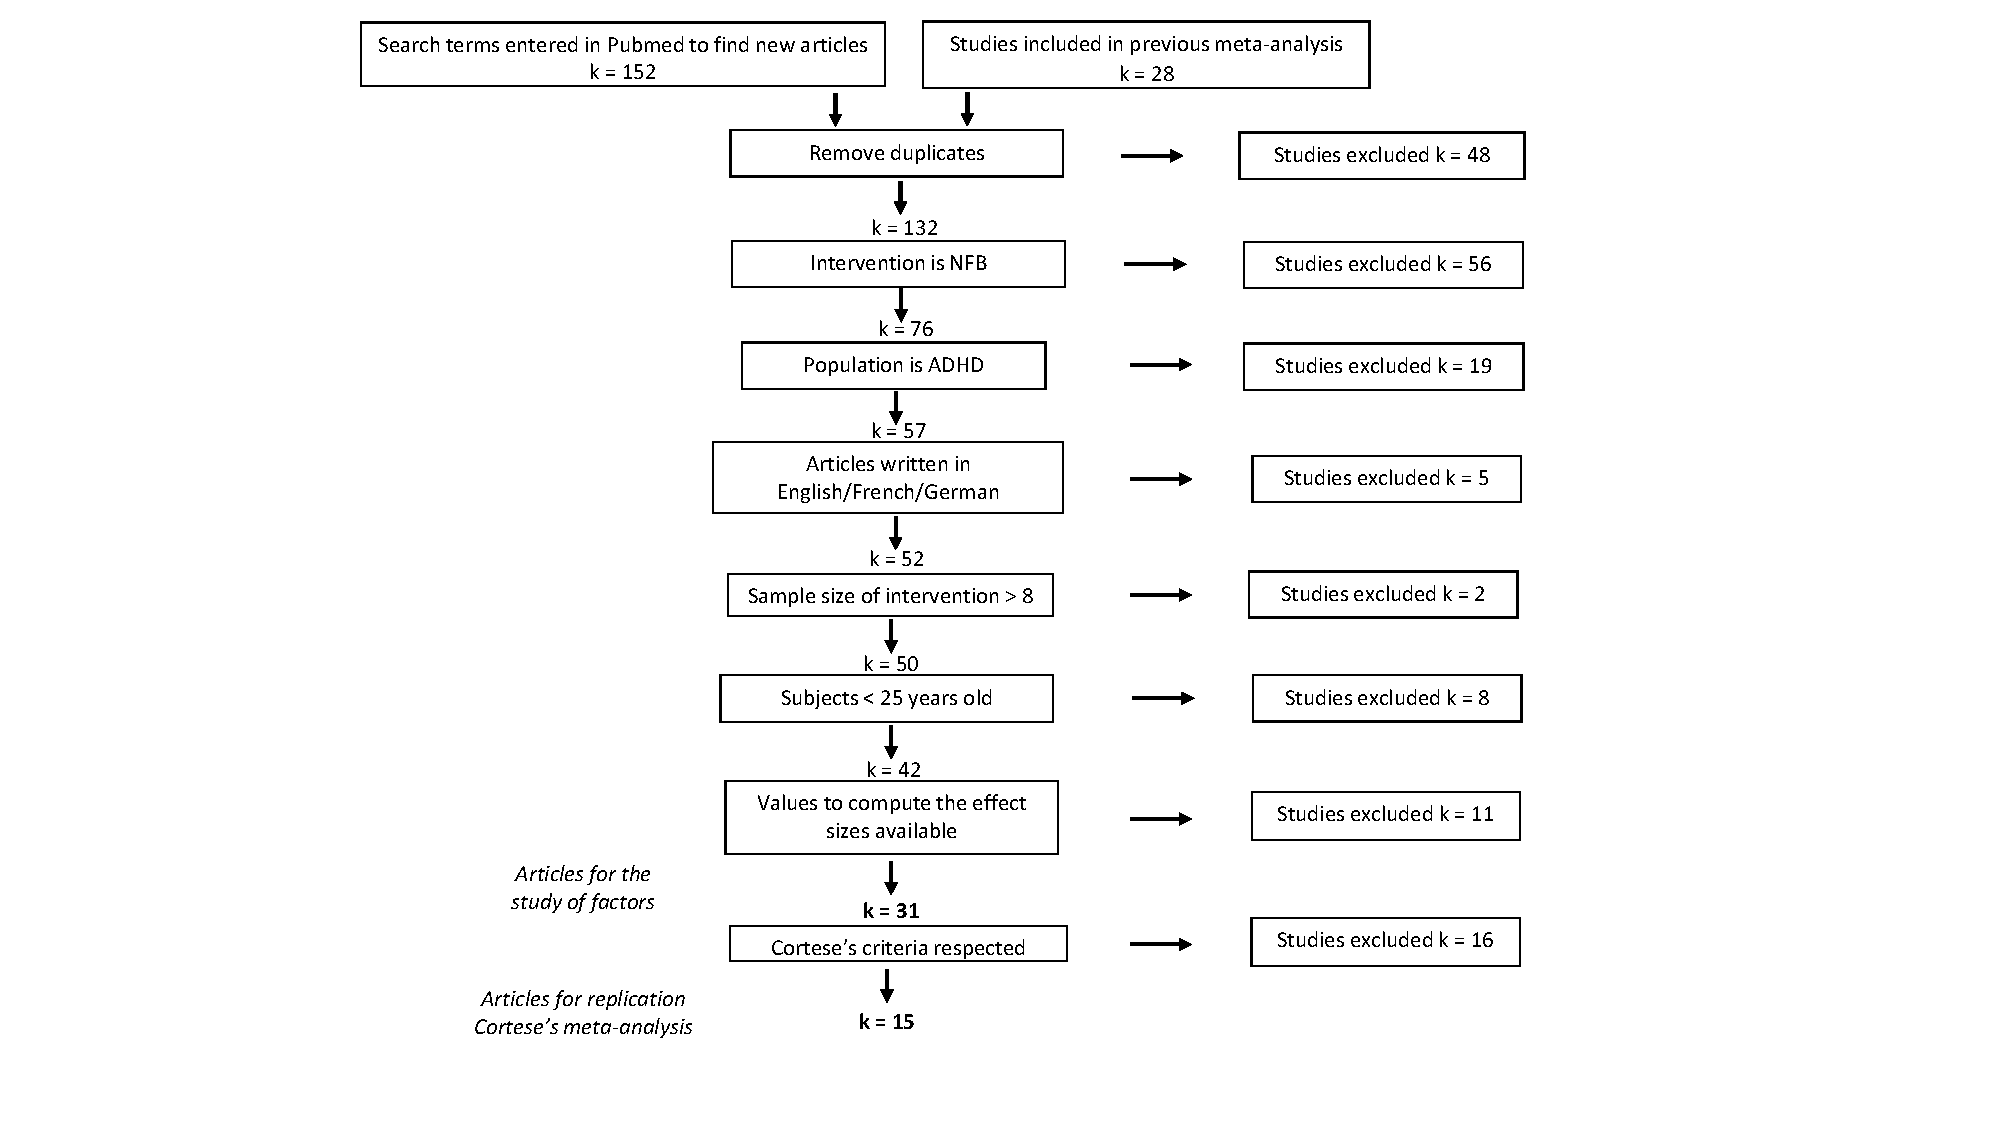
\includegraphics[width=1.0\linewidth]{figures/meta_review_factors_analysis_how_studies_are_included_no_colors_2-columns_fitting_ima}
  \caption{Flow diagram of selection of studies (last search on December 14, 2017).}
  \label{Figure:systematic_review_workflow}
\end{figure}

\subsection{Replicate a meta-analysis}

Contrary to \citet{Cortese2016}, the Python code returns a negative \gls{es} when the clinical trial is in favor of \gls{nfb}. 
The \gls{se} whose p-value $<$ 0.05 was considered statistically significant. 

First, when using the \gls{es} found by \citet{Cortese2016} thanks to RevMan \citep{RevMan}, and then performed the following steps 
of meta-analysis with the Python code, we observe no major differences between these results and those obtained with RevMan \citep{RevMan} 
as listed in \cref{Table:meta_review_comparison_between_revman_python}. The minor discrepancies, especially observed at the p-values level,
 are due to our choice to always use a pre-post correlation of 0.5 when computing the variance of each \gls{es}. Moreover, a sensitivity 
analysis was conducted to ensure the minor impact of the pre-post correlation value: when it varies between 0.2 and 0.8 the significance 
of the \gls{se} does not change. 

\begin{table}[h!]
  \centering
  \caption{Comparison between \citet{Cortese2016} results obtained with RevMan \citep{RevMan} and those obtained with the Python code. Summary 
	effects and their corresponding p-value in parenthesis are presented. With the Python program, a negative summary effect is in favor of \gls{nfb}.}
\begin{tabular}{ |p{2cm}|p{2.5cm}|p{4cm}|p{4.5cm}|  }
\hline
 \multicolumn{2}{ |c| }{Input data} & Results from \citet{Cortese2016} & Effect sizes from \citet{Cortese2016}\\
\hline
\multicolumn{2}{ |c| }{Implementation} & RevMan \citet{RevMan} & Python program\\
\hline
\multirow{3}{*}{ \textit{Parents} } & Total & $0.35$ ($0.004$) & $-0.34$ ($0.004$)\\
 & Inattention  & $0.36$ ($0.009$) & $-0.35$ ($0.011$)\\
 & Hyperactivity  & $0.26$ ($0.004$) & $-0.24$ ($0.02$)\\
\hline
\multirow{3}{*}{ \textit{Teachers} } & Total & $0.15$ ($0.20$) & $-0.13$ ($0.25$)\\
 & Inattention  & $0.06$ ($0.70$) & $-0.09$ ($0.50$)\\
 & Hyperactivity  & $0.17$ ($0.13$) & $-0.15$ ($0.21$)\\
 \hline
\end{tabular}

  \label{Table:meta_review_comparison_between_revman_python}
\end{table}

Thanks to the previous step, we can conclude that the Python code yields results close to those returned by RevMan \citet{RevMan}, so all 
the following results were computed with the Python code. 

The replication of \citet{Cortese2016} was conducted by applying the following choices and the results obtained are presented 
in \cref{Table:meta_review_comparison_revman_and_python_with_choices}:

\begin{description}
    \item To compute the \gls{es} for \citet{Arnold2014}, \citet{Cortese2016} took as post-test values the assessments after 12 \gls{nfb} sessions
		because results at post-test were not available. In our case, we used the values at post-test (i.e after the 40 sessions). With these values, 
		we find smaller \gls{es} than \citet{Cortese2016}.  
    \item Different results for teachers' assessments were found for \cite{Steiner2014} because we decided not to use the same scale 
		as \citet{Cortese2016}. Indeed, \citet{Cortese2016} relied on the BOSS Classroom Observation \citep{Shapiro2010} to compute \gls{es}
		for teachers' ratings even if this scale is not as used as other scales provided in this study. That's why we decided to conduct our analysis
		with a more common scale which has been part of studies assessing the pros and cons of different ADHD scales \citep{Epstein2012, Collett2003}: The Conners. 
		Besides, this scale was already used in this study to compute the \gls{es} for the parents' ratings. 
		Using this scale leads to higher \gls{es} in attention but not in total and hyperactivity. Moreover, this different choice of 
		scale does not affect the significance of the summary effects.
		\item Eventually, there is a slight overall difference between \gls{es} computed by \citet{Cortese2016} and those yielded by our Python 
		code maybe due to the fact that the correcting factor for small sample $cp$ is not applied in our work. Besides, as mentioned earlier, 
		there is a little difference in some \gls{es}' standard error explained by the use of a pre-post correlation value  of 0.5 
		while computing the variance of the \gls{es}. These two discrepancies does not change the significance of the summary effect.
\end{description}

\begin{table}[h!]
  \centering
  \caption{Comparison between \citet{Cortese2016} results obtained with RevMan \citep{RevMan} and those obtained with the Python code with our 
	choices applied. Summary effects and their corresponding p-value (in parenthesis) are presented. With the Python program, a negative summary 
	effect is in favor of \gls{nfb}.}
\begin{tabular}{cccc}

\toprule
\multicolumn{2}{c}{Input data} & \shortstack{ Results from \\ \citet{Cortese2016} \\ (for reference)} & \shortstack{ Means and standard \\ deviations from \\ articles included in \\ \citet{Cortese2016} }\\
\midrule
\multicolumn{2}{c}{Implementation} & \shortstack{ RevMan \\ \citet{RevMan} } & Python program\\
\midrule
\multicolumn{2}{ c }{Hypothesis} & \shortstack{ Same as \\ \citet{Cortese2016} } & Our choices$^a$\\
\midrule
\multirow{ 3}{*}{ \textit{Parents} } & Total & $0.35$ ($0.004$) & $-0.32$ ($0.013$)\\
 & Inattention  & $0.36$ ($0.009$) & $-0.31$ ($0.036$)\\
 & Hyperactivity  & $0.26$ ($0.004$) & $-0.24$ ($0.02$)\\
\multirow{ 3}{*}{ \textit{Teachers} } & Total & $0.15$ ($0.20$) & $-0.11$ ($0.37$)\\
 & Inattention  & $0.06$ ($0.70$) & $-0.17$ ($0.16$)\\
 & Hyperactivity  & $0.17$ ($0.13$) & $-0.022$ ($0.85$)\\
\bottomrule

\end{tabular}

  \label{Table:meta_review_comparison_revman_and_python_with_choices}
\end{table}

\subsection{Update a meta-analysis}

The next step consisted in extend \citet{Cortese2016} meta-analysis by adding the two new articles \citep{Strehl2017, Baumeister2016} found 
during the systematic review. \citet{Baumeister2016} provided results only for parents total outcome whereas \citet{Strehl2017} gave teachers 
and parents' assessments for all outcomes. In spite of favorable results for \gls{nfb}, particularly on parents' assessments, adding these two 
new studies does not change either the magnitude or the significance of the summary effect for any outcome whatever the raters or the choices made 
as summed up in \cref{Table:meta_review_comparison_revman_plus_new_and_python_new_plus_with_choices}.
 
\clearpage
\begin{landscape}
\begin{table}[h!]
\centering
\caption{Comparison between \citet{Cortese2016} results obtained with RevMan \citep{RevMan} with and without the two new articles and 
those obtained with the Python code with our choices applied plus the two new articles. Summary effects and their corresponding p-value 
(in parenthesis) are presented. With the Python program, a negative summary effect is in favor of \gls{nfb}.}
\begin{tabular}{ |p{2cm}|p{2.5cm}|p{4cm}|p{4.5cm}|p{4.5cm}|  }
\hline
\multicolumn{2}{ |c| }{Input data} & Results from \citet{Cortese2016} & Results from \citet{Cortese2016} and means and standard deviations from the new two articles & Means and standard deviations from articles included in \citet{Cortese2016} and the two new studies\\
\hline
\multicolumn{2}{ |c| }{Implementation} & RevMan \citet{RevMan} & Effect sizes: RevMan \citet{RevMan} and then Python program & Python program\\
\hline
\multicolumn{2}{ |c| }{Hypothesis} & Same as \citet{Cortese2016} & Same as \citet{Cortese2016} & Our choices\\
\hline
\multirow{ 3}{*}{ \textit{Parents} } & Total & $0.35$ ($0.004$) & $0.37$ ($0.0004$) & $-0.34$ ($0.0017$) \\
 & Inattention  & $0.36$ ($0.009$) & $0.37$ ($0.0015$) & $-0.33$ ($0.011$)\\
 & Hyperactivity  & $0.26$ ($0.004$) & $0.24$ ($0.002$) & $-0.23$ ($0.0094$)\\
\hline
\multirow{ 3}{*}{ \textit{Teachers} } & Total & $0.15$ ($0.20$) & $0.14$ ($0.15$) & $-0.11$ ($0.27$)\\
 & Inattention  & $0.06$ ($0.70$) & $0.06$ ($0.66$) & $-0.14$ ($0.17$)\\
 & Hyperactivity  & $0.17$ ($0.13$) & $0.16$ ($0.96$) & $-0.05$ ($0.6$)\\
\hline
\end{tabular}

 
  \label{Table:meta_review_comparison_revman_plus_new_and_python_new_plus_with_choices}
\end{table}
\end{landscape}

Next, we ran the analysis on two specific subgroups: on the one hand only studies following standard protocol defined by \citet{Arns2014}
are selected and on the other hand only studies forbidding participants to take medication during the clinical trial are included. 

Regarding the standard protocol subgroup, \citet{Cortese2016} found all the outcomes significant except for the hyperactivity symptoms 
rated by teachers. However, when adding \citep{Strehl2017} results, we find no significance for the inattention symptoms assessed by 
teachers as well (p-value = 0.10 when following \citeauthor{Cortese2016}'s choices and 0.11 with our choices). 
As for the low/no medication subgroup, summary effects are not significant except for the inattention symptoms assessed by parents (p-value = 0.013). 
Besides, the differences in \citet{Arnold2014} values causes a loss of significance in 
hyperactivity outcome for parents (p-value = 0.066) compared to \citet{Cortese2016} (p-value = 0.016). The two new studies were not included in this subgroup because 
subjects are taking psychostimulants during the trial.

All the scales used to compute the effect sizes following our choices are summarized in Supplemental material.

\subsection{Detect factors influencing the Neurofeedback}

This analysis was performed on 31 trials assessing the efficacy of \gls{nfb} as presented in \cref{Table:table_factors_analysis_list_of_included_studies}. 
Among the 25 factors selected, 6 were removed because there were either too many missing observations or they were too homogeneous: beta up frontal, 
the use of a transfer card, the type of threshold for the rewards (incremental or fixed), the EEG quality equal to 3 and presence of a control group. 

To assess the variability of each factor, box plots of their standardized values were displayed in \cref{Figure:factors_analysis_boxplots}: treatment length, 
session length and number of sessions are more variable across studies than session pace, minimum and maximum age.      

\begin{table}[h!]
  \centering
  \caption{List of included studies to perform the factors analysis.}
  \begin{tabular}{ cccc }
\toprule
Trial & Year & \shortstack{ Size of the \\ \gls{nfb} group } & Weight \\
\hline
\citeauthor{Arnold2014} & 2014 & 26 & 6.5\\ 
\citeauthor{Bakhshayesh2011} & 2011 & 18 & 9\\
\citeauthor{Baumeister2016} & 2016 & 8 & 8\\
\citeauthor{Bakhshayesh2011} & 2011 & 18 & 9\\
\citeauthor{Beauregard2006} & 2006 & 15 & 15\\
\citeauthor{Bink2014} & 2014 & 45 & 15\\
\citeauthor{Bluschke2016} & 2016 & 19 & 19\\
\citeauthor{Christiansen2014} & 2014 & 14 & 7\\
\citeauthor{Deilami2016} & 2016 & 12 & 12\\
\citeauthor{Drechsler2007} & 2007 & 17 & 5.67\\
\citeauthor{Duric2012} & 2012 & 23 & 23\\
\citeauthor{Escolano2014} & 2014 & 20 & 20\\
\citeauthor{Gevensleben2009} & 2009 & 59 & 14.75\\
\citeauthor{Heinrich2004} & 2004 & 13 & 13\\
\citeauthor{Holtmann2009} & 2009 & 20 & 20\\
\citeauthor{Kropotov2005} & 2005 & 86 & 86\\
\citeauthor{Lee2017} & 2017 & 18 & 6\\
\citeauthor{Leins2007} & 2007 & 19 & 19\\
\citeauthor{Li2013} & 2013 & 20 & 10\\
\citeauthor{Linden1996} & 1996 & 9 & 9\\
\citeauthor{Maurizio2014} & 2014 & 13 & 3.25\\
\citeauthor{Meisel2014} & 2014 & 12 & 6\\
\citeauthor{Mohagheghi2017} & 2017 & 30 & 30\\
\citeauthor{Mohammadi2015} & 2015 & 16 & 16\\
\citeauthor{Monastra2002} & 2002 & 51 & 51\\
\citeauthor{Ogrim2013} & 2013 & 13 & 6.50\\
\citeauthor{Steiner2011} & 2011 & 9 & 2.25\\
\citeauthor{Steiner2014} & 2014 & 34 & 6.80\\
\citeauthor{Strehl2006} & 2006 & 23 & 5.75\\
\citeauthor{Strehl2017} & 2017 & 72 & 16.25\\
\citeauthor{VanDongen2013} & 2013 & 22 & 11\\
\bottomrule
\end{tabular}

  \label{Table:table_factors_analysis_list_of_included_studies}
\end{table}

\begin{figure}[h!]
  \centering
  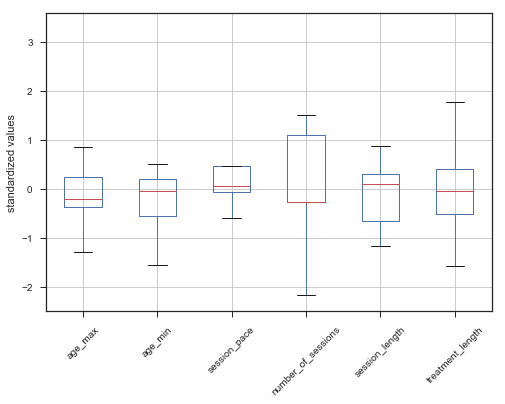
\includegraphics[scale=0.5]{figures/factors_analysis_boxplot_no_colors_no_two_columns}
  \caption{Boxplots of the standardized values of each continuous factor.}
  \label{Figure:factors_analysis_boxplots}
\end{figure}

The first method used to detect the influencing factors was the \gls{wls}. First, the assumptions inherent to this method were checked: 
\begin{description}
	\item the moment matrix $\mathbf{{X}^{T}W^{T}WX}$ was invertible;
  \item no apparent correlation between the continuous independent variables was found; 
  \item the fit was significant as shown by the F-statistic (prob(F-statistic) = 2.21e-10); 
  \item the residuals were normally distributed as demonstrated by the skew (-0.166), kurtosis (2.85) and the Omnibus test (prob(Omnibus) = 0.84).
\end{description}

Since these assumptions are satisfied, we can be rather confident in the \gls{wls} results presented in \cref{Table:factors_analysis_wls_results}. 
We find that 8 factors are significantly different from zero for an adjusted R-squared of 0.74. When applying the \gls{ols} the assumptions of the 
model are satisfied too and the same factors are returned as significant except the transfer phase, 
the protocol theta down and the artifact correction based on amplitude with an adjusted R-squared of 0.42. 

\begin{table}[h!]
  \centering
  \caption{Results of the \gls{wls}. A p-value $<$ 0.05 means that the coefficient of the corresponding factor is significantly different from $0$ (in bold). 
	When the value of the coefficient is negative, the corresponding factor may lead to better \gls{nfb} results.}
  \begin{center}
\begin{tabular}{ |p{4cm}|p{4cm}|p{4cm}|p{2cm}|}
\hline
\multicolumn{2}{ |c| }{Independent variables (factors)} & Value of the coefficient & p-value\\
\hline
\multirow{ 2}{*}{ \textit{Signal quality} } & \gls{eog} correction & $-0.081$ & $0.40$\\ 
& \textbf{artifact correction based on amplitude} & $0.15$ & $0.039$\\ 
\hline
\multirow{ 3}{*}{ \textit{Methodological} } & \textbf{\gls{pblind}} & $0.11$ & $0.038$\\ 
& randomization & $0.0099$ & $0.89$\\ 
& \textbf{\gls{irb}} & $-0.30$ & $0.00$\\ 
\hline
\multirow{ 3}{*}{ \textit{Population} } & age max & $-0.087$ & $0.17$\\
& age min & $-0.050$ & $0.43$\\
& on drugs & $0.065$ & $0.45$\\
\hline
\multirow{ 9}{*}{ \textit{\gls{nfb} implementation} } & number of sessions  & $-0.015$ & $0.84$\\
& session length & $0.17$ & $0.18$\\
& \textbf{session pace} & $-0.25$ & $0.00$\\ 
& \textbf{treatment length} & $0.57$ & $0.00$\\
& \gls{smr} & $-0.067$ & $0.38$\\ 
& beta up central & $-0.025$ & $0.73$\\  
& \textbf{theta down} & $-0.29$ & $0.019$\\
& \gls{scp} & $-0.90$ & $0.54$\\
& \textbf{transfer phase} & $0.27$ & $0.030$\\
\hline
\multirow{ 2}{*}{ \textit{Quality of acquisition} } & more than one active electrode & $0.0639$ & $0.359$\\ 
& \textbf{\gls{eeg} quality 2} & $-0.36$ & $0.00$\\ 
\hline
\end{tabular}
\end{center}
  \label{Table:factors_analysis_wls_results}
\end{table}

A negative coefficient meant that the factor was in favor of the \gls{nfb}. Here, among the factors whose coefficient is significantly 
different from 0, a long treatment, a blind rater, including a transfer phase, and correcting artifact thanks to the amplitude appear 
to have a negative influence on the \gls{nfb} performance. Conversely, an \gls{irb} approval, a high number of sessions per week, a theta
down protocol and an EEG quality of 2 seem to lead to more efficacy. 

Next, a \gls{lasso} regression was conducted in order to perform variables selection among the factors. As the first step, the tuning 
parameter $\lambda$ was obtained by leave one out cross validation. 
$\lambda$ corresponds to the abscissa of the minimum of the \gls{mse} on the mean fold computed on $\lambda$ values ranging from very 
small to very big, covering the full range of scenarios from the null model to the least square fit.

The penalty applied leads to the selection of 12 factors as summed up in \cref{Table:table_factors_analysis_lasso_results}.
\begin{table}[h!]
  \centering
  \caption{Results of the \gls{lasso}. Factors different from 0 are selected (in bold). When the value of the coefficient is negative, the corresponding 
	factor may lead to better \gls{nfb} results.}
  \begin{center}
\begin{tabular}{ |p{4cm}|p{4cm}|p{4cm}|}
\hline
\multicolumn{2}{ |c| }{Independent variables (factors)} & Value of the coefficient\\
\hline
\multirow{ 2}{*}{ \textit{Signal quality} } & \gls{eog} correction & $0.00$\\ 
& \textbf{artifact correction based on amplitude} & $0.047$\\ 
\hline
\multirow{ 3}{*}{ \textit{Methodological} } & \textbf{\gls{pblind}} & $0.11$\\ 
& \textbf{randomization} & $0.032$\\  
& \textbf{\gls{irb}} & $-0.15$\\  
\hline
\multirow{ 3}{*}{ \textit{Population} } & age max & $0.00$\\
& age min & $0.00$\\
& \textbf{on drugs} & $0.032$\\
\hline
\multirow{ 9}{*}{ \textit{\gls{nfb} implementation} } & number of sessions  & $0.00$\\
& session length & $0.00$\\ 
& \textbf{session pace} & $-0.14$\\ 
& \textbf{treatment length} & $0.33$\\ 
& \textbf{\gls{smr}} & $0.061$\\
& beta up central & $0.00$\\  
& \textbf{theta down} & $-0.051$\\
& \textbf{\gls{scp}} & $0.10$\\ 
& \textbf{transfer phase }& $0.11$\\
\hline
\multirow{ 2}{*}{ \textit{Quality of acquisition} } & more than one active electrode & $0.00$\\ 
& \textbf{\gls{eeg} quality 2} & $-0.23$\\  
\hline
\end{tabular}
\end{center}

  \label{Table:table_factors_analysis_lasso_results}
\end{table}

With this method, a negative coefficient corresponds also to favorable factors. Thus, having several sessions per week, being approved 
by an \gls{irb}, a protocol theta down, and an EEG quality of 2 seem to improve the results of the \gls{nfb}. 
On the contrary, a blind rater, a long treatment, randomizing the groups, a \gls{scp} and \gls{smr} protocols, being on drugs during the trial, correcting 
artifact based on the amplitude of the signal, and including a transfer phase during the session appear to be factors with a negative influence.

Eventually, the decision tree presented in \cref{Figure:factors_analysis_decision_tree_results} splits the dataset based on the factor leading to the
 smallest \gls{mse}. The best predictor is the one at the top of the tree: in our case it is the \gls{pblind}. So, the dataset is divided in two subsets: 
43 samples where the assessments were reported by non-blind raters and 19 samples based on blind ratings. This last subset, where the \gls{se} is smaller 
than the one obtained for non-blind raters, is split on the age min criteria: it appeares that the lower the age, the better the results. Regarding 
the side of the tree where the raters are non-blind, the next factor leading to the smallest \gls{mse} is the treatment length. A smaller treatment
 length seems to lead to better \gls{nfb} results. In that case, the EEG quality 2 enables to break down the subset and according to these results
 if this factor is respected in studies it seems to lead to higher \gls{se}. The lower we get into the tree, the less samples are available, so results 
were less and less reliable.

\begin{figure}[h!]
  \centering
  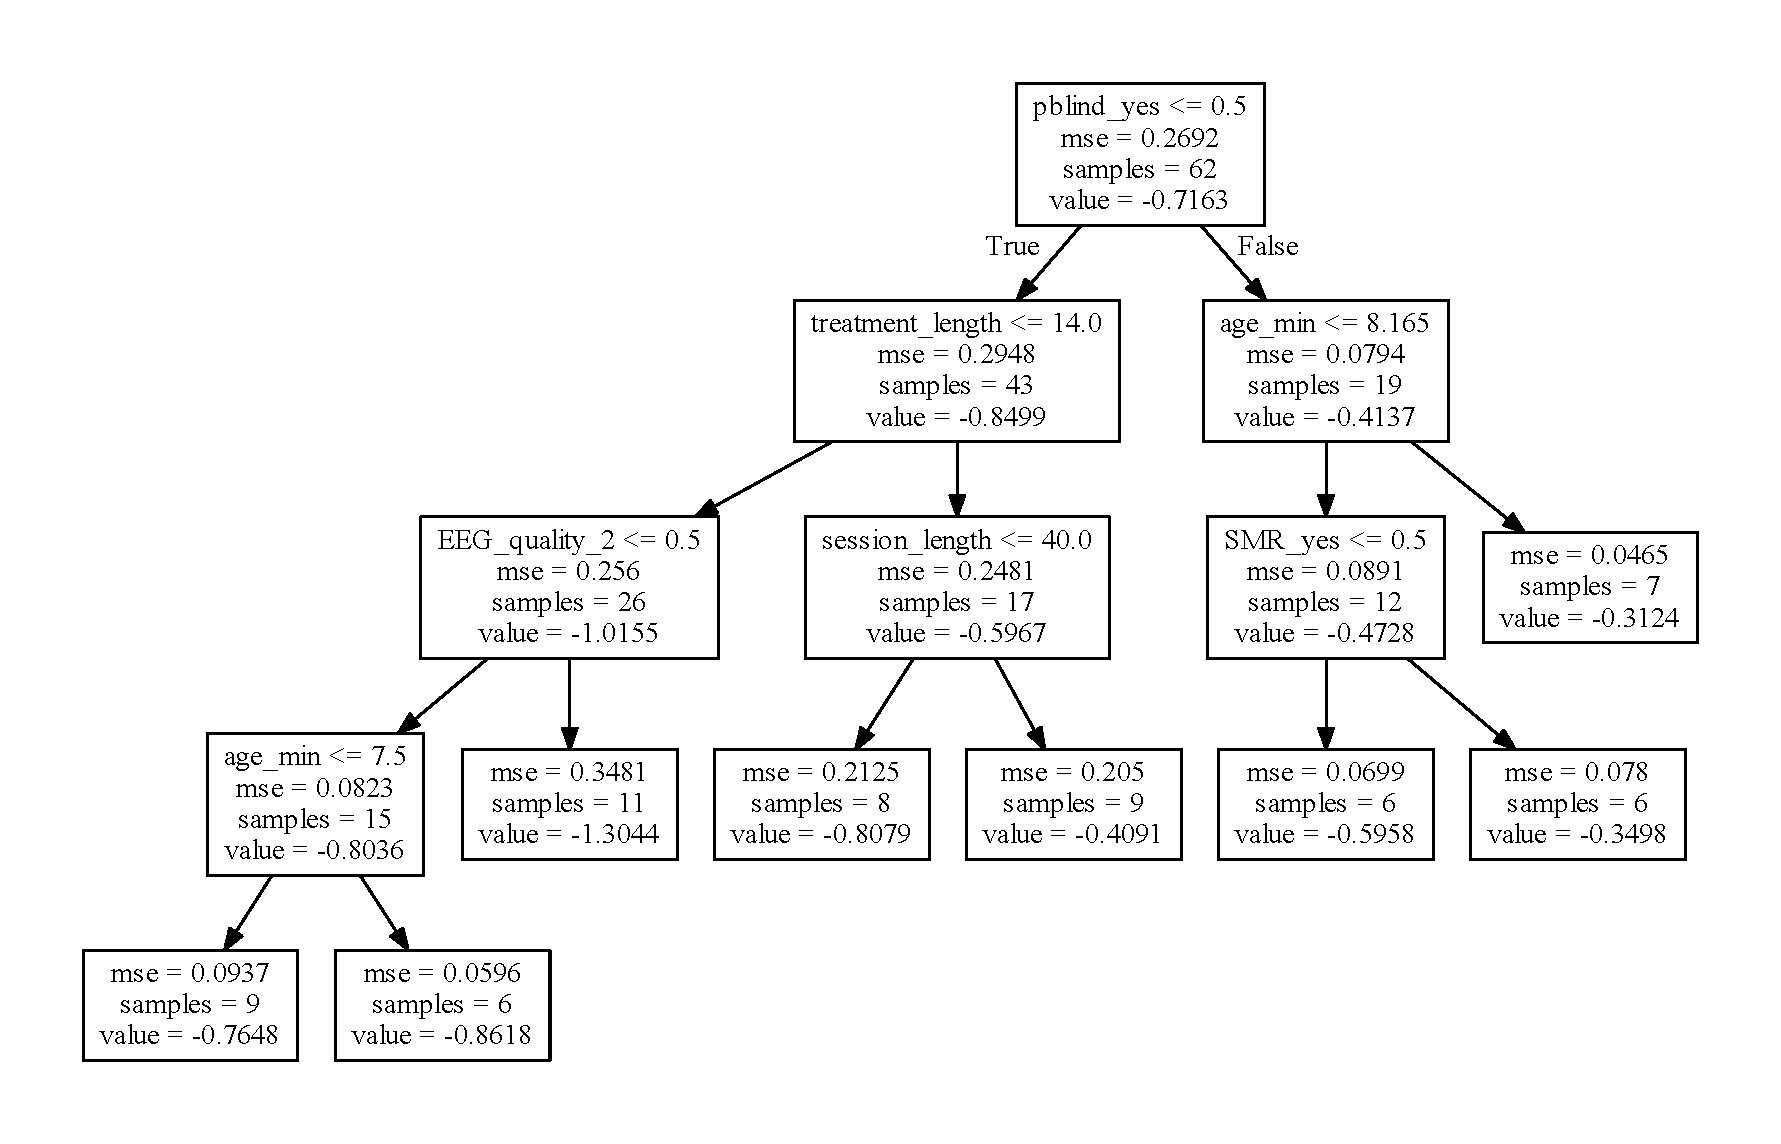
\includegraphics[width=1.0\linewidth]{figures/factors_analysis_decision_tree_results_no_colors_2-columns_fitting_image}
  \caption{Decision Tree obtained with the factors. The criteria to minimize was the \gls{mse}. For the dummy variables, a value of $1$ meant
	that the factor was observed in the study. The value corresponded to the value of the dependent variable.}
  \label{Figure:factors_analysis_decision_tree_results}
\end{figure}

The different methods do not detect exactly the same factors but many are common as presented in \cref{Table:table_factors_analysis_results_summary},
 in particular the treatment length, the assessment by a blind rater and \gls{eeg} quality of 2 which are returned by the three methods. Besides, 
the methods agree on the direction of the influence of these factors. However, it is more difficult to interpret the influence of the factors 
returned only by one or two methods. For instance, both \gls{wls} and \gls{lasso} find that  
relying on the amplitude of the signal to correct artifacts, and including a transfer phase seem not to improve the \gls{adhd} symptoms. 
However, the \gls{irb} approval, a theta down protocol, and a high number of sessions per week appear to 
positively influence the results. The decision tree and \gls{lasso} have in common the protocol \gls{smr}: it is associated with lower \gls{es}.
Five factors are returned by only one of the methods: the minimal age of the children, being on drugs 
during \gls{nfb} treatment, randomizing the groups and the \gls{scp} protocol.  

\begin{table}[h!]
  \centering
  \caption{Summary of the results obtained with the three methods. The type of sign describes the direction of the influence on the \gls{nfb} 
	results ($+$ for a positive effect and a $-$ for a negative one). The number of signs illustrates the number of methods who finds the factor 
	as influencing. Factors returned by 3, 2 and 1 methods influence the \gls{nfb} with respectively high, moderate and poor confidence.}
  \begin{center}
\begin{tabular}{ p{3cm} p{3cm} p{3cm} p{2cm} p{2cm} p{2cm}}
\toprule
\multicolumn{2}{c}{ \shortstack{Independent \\ variables (factors)} } & \shortstack{ \gls{wls} \\ (p-value) } & \gls{lasso} & \shortstack{Decision \\ Tree} \\
\midrule
\multirow{ 2}{*}{ \textit{Signal quality} } & \gls{eog} correction & \hskip 0.08in-0.078 (0.41) &  \hskip 0.12in0.00 & / \\ 
& artifact correction based on amplitude & \hskip 0.12in\textbf{0.15(0.040)} & \hskip 0.12in\textbf{0.047} & / \\ 
\midrule
\multirow{ 3}{*}{ \textit{Methodological} } & \gls{pblind} & \hskip 0.12in\textbf{0.10 (0.043)} & \hskip 0.12in\textbf{0.11} & \textbf{selected} \\ 
& randomization & \hskip 0.12in0.0069 (0.92) & \hskip 0.12in\textbf{0.032} & / \\  
& \gls{irb} & \hskip 0.08in\textbf{-0.29 (0.00)} & \hskip 0.08in\textbf{-0.15} & / \\  
\midrule
\multirow{ 3}{*}{ \textit{Population} } & age max & \hskip 0.08in-0.090 (0.16) & \hskip 0.12in0.00 & / \\
& age min & \hskip 0.08in-0.055 (0.37) & \hskip 0.12in0.00 & \textbf{selected }\\
& on drugs & \hskip 0.12in0.069 (0.42) & \hskip 0.12in\textbf{0.032} & / \\
\midrule
\multirow{ 9}{*}{ \textit{ \shortstack{\gls{nfb} \\ implementation} } } & number of sessions  & \hskip 0.08in-0.0075 (0.92) & \hskip 0.12in0.00 & / \\
& session length & \hskip 0.12in0.17 (0.17) & \hskip 0.12in0.00 & \textbf{selected} \\
& treatment length & \hskip 0.12in\textbf{0.57 (0.00)} & \hskip 0.12in\textbf{0.33} & \textbf{selected} \\
& session pace & \hskip 0.08in\textbf{-0.25 (0.00)} & \hskip 0.08in\textbf{-0.14} & / \\ 
& \gls{smr} & \hskip 0.08in-0.063 (0.41) & \hskip 0.12in\textbf{0.061} & \textbf{selected} \\
& beta up central & \hskip 0.08in-0.027 (0.72) & \hskip 0.12in0.00 & / \\  
& theta down & \hskip 0.08in\textbf{-0.29 (0.014)} & \hskip 0.08in\textbf{-0.051} & / \\
& \gls{scp} & \hskip 0.08in-0.099 (0.50) & \hskip 0.12in\textbf{0.10} & / \\ 
& transfer phase & \hskip 0.12in\textbf{0.27 (0.032)} & \hskip 0.12in\textbf{0.11} & / \\
\midrule
\multirow{ 2}{*}{ \textit{ \shortstack{Quality of \\ acquisition} } } & more than one active electrode & \hskip 0.12in0.064 (0.36) & \hskip 0.12in0.00 & / \\ 
& \gls{eeg} quality 2 & \hskip 0.08in\textbf{-0.36 (0.00)} & \hskip 0.08in\textbf{-0.23} & \textbf{selected} \\  
\bottomrule
\end{tabular}
\end{center}

  \label{Table:table_factors_analysis_results_summary}
\end{table}

% words number = 1635